\section{Introduction}

% What is the problem?
File system metadata services in HPC have scalability problems. It has been
shown that HPC workloads are metadata resource intensive because administrative
tasks, like checkpointing~\cite{bent_plfs_2009} or scanning the file
system~\cite{zheng:pdsw2014-batchfs}, on large data sets leads to contention
for the same directories and inodes ({\it
e.g.}, path traversal). Applications perform better with dedicated metadata
servers~\cite{sevilla:sc15-mantle, ren:sc2014-indexfs} but provisioning a
metadata server for every client is unreasonable. This problem is exacerbated
by current trends in HPC, where architectures are transitioning from complex
storage stacks with burst buffer, file system, object store, and tape tiers to
more simplified stacks with just a burst buffer and object
store~\cite{bent:login16-hpc-trends}; this puts more pressure on data access
because more requests end up hitting the same layer and latencies cannot be 
hidden while data migrates across tiers.

\begin{figure}[tb]
\centering
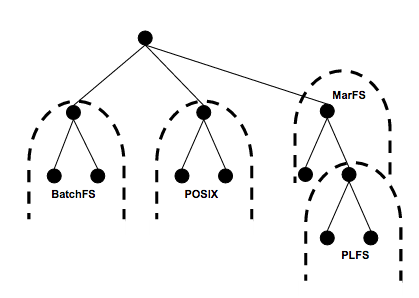
\includegraphics[width=0.5\textwidth]{figures/subtree-policies.png}
\caption{Users can assign weaker consistency and durability policies
to subtrees to get the same performance benefits of state-of-the-art HPC
architectures. Applications that need stronger guarantees can still reside in
the same namespace.
}\label{fig:subtree-policies}
\end{figure}


% What is HPC doing?
To address this, developers are relaxing the consistency and durability
semantics in the file system because weaker guarantees are sufficient for their
applications. For example, batch style jobs often do not need the strong
consistency that the file system provides, so
BatchFS~\cite{zheng:pdsw2014-batchfs} and DeltaFS~\cite{zheng:pdsw2015-deltafs}
do more client-side processing and merge updates when the job is done. HPC
developers are turning to these non-POSIX solutions because their applications
are well-understood ({\it e.g.}, well-defined read/write phases,
synchronization only needed during certain phases, workflows describing
computation, etc.) and because they wreak havoc on file systems designed for
general-purpose workloads ({\it e.g.}, checkpoint-restart's N-N and N-1 create
patterns).

% One example
One popular approach for relaxing consistency and durability is to ``decouple
the namespace", where clients lock the subtree they want exclusive access to as
a way to tell the file system that the subtree is important or may cause
resource contention in the near-future~\cite{grider:pdsw2015-marfs,
zheng:pdsw2015-deltafs, zheng:pdsw2014-batchfs, ren:sc2014-indexfs,
bent:slides-twotiers}. Then the file system can change its internal structure
to optimize performance. For example, the file system could enter a mode that
prevents other clients from interferring with the decoupled directory.  This
delayed merge ({\it i.e.} a form of eventual consistency) and relaxed
durability improves performance and scalability by avoiding the costs of RPCs,
synchronization, false sharing, and serialization.  The consistency and
durability semantics for these systems is shown in
Figure~\ref{fig:subtree-policies} (table) . While the performance benefits are obvious
for these users, applications that rely on the file system's guarantees must be
deployed on an entirely different system or re-written to coordinate strong
consistency/durability themselves.

%\begin{table}
%\begin{tabular}{ r | l }
%  Subtree         & Example \\\hline
%  (1)   & \{Index, Batch\}FS~\cite{ren:sc2014-indexfs, zheng:pdsw2014-batchfs} \\
%  (2)   & \{Index, Ceph\}FS~\cite{ren:sc2014-indexfs, weil:sc2004-dyn-metadata} \\
%  (3)   & RAMDisk \\
%  (4)   & DeltaFS~\cite{zheng:pdsw2015-deltafs} \\
%\end{tabular}
%
%\caption{State-of-the-art systems in HPC improve file system metadata
%performance by relaxing consistency and durability guarantees. Note that
%IndexFS also supports weak consistency with bulk inserts.
%\label{table:namespaces}} \end{table}

% What did we do
We propose a subtree policy API that lets future programmers control
the consistency and durability for subtrees in the file system namespace. For performance, one
subtree can adopt weaker consistency semantics while another subtree can retain
the rigidity of POSIX's strong consistency. Figure~\ref{fig:subtree-policies}
shows an example setup where a single global namespace has directories for
applications designed for different, state-of-the-art HPC architectures.  We
present Cudele, a prototype programmable file system that supports different
degrees of consistency and durability by exposing mechanisms used within the
file system as a client library.  CudeleFS supports 3 forms of consistency
(invisible, weak, and strong) and 3 degrees of durability (none, local, and
global) giving the user a wide range of policies and optimizations
that can be custom fit to an application. Our contributions: 

\begin{enumerate}

  \item a prototype that lets users program a range of
  consistency and durability semantics (9 permutations), allowing them to custom
  fit the storage system to the application.

  \item an API for programming consistency/durability policies and assigning
  them to subtrees in the file system namespace.

  \item an apples-to-apples comparison of the strategies used in recently proposed research systems against
  previously unexplored metadata designs, all implemented using Cudele.

\end{enumerate}

% Results
Our results confirm the assertions of ``clean-state" research systems that
decouple namespaces; specifically that the technique drastically improves
performance (104\(\times\) speed up) but we go a step further by quantifying
the costs of merging updates (7\(\times\) slow down) and maintaining durability
(\(10\times\) slow down). We also show the effect of having a metadata specific
file format in systems that are based on in-memory data structures.
Section~\ref{sec:posix-overheads} quantifies the cost of POSIX
consistency and system-defined durability and
Section~\ref{sec:methodology-decoupled-namespaces} presents the Cudele
prototype and API. Section~\ref{sec:implementation} describes Cudele's
mechanisms and shows how re-using internal subsystems results in an
implementation of less than 500 lines of code. The evaluation in
Section~\ref{sec:evaluation} quantifies the overheads and performance gains of
explored and previously unexplored metadata designs.
Section~\ref{sec:related-work} places CudeleFS in the context of other related
work.

